\documentclass[svgnames]{article}
\usepackage[utf8]{inputenc}
\usepackage{amsmath}
\usepackage{amssymb}
\usepackage{mathrsfs}
\usepackage{mathtools}
\newtheorem{mydef}{Given}
\newtheorem{mytheorem}{Theorem}
\usepackage{enumitem}
\usepackage{venndiagram}
\usepackage{smartdiagram}
\usepackage{caption}
\usepackage{subcaption}
%\usepackage[framed,numbered,autolinebreaks,useliterate]{mcode}
\usepackage{pgfplots}
%\usepackage{tkiz}



\usepackage{listings}
\usepackage{color}

\definecolor{dkgreen}{rgb}{0,0.6,0}
\definecolor{gray}{rgb}{0.5,0.5,0.5}
\definecolor{mauve}{rgb}{0.58,0,0.82}

\lstset{frame=tb,
  language=Java,
  aboveskip=3mm,
  belowskip=3mm,
  showstringspaces=false,
  columns=flexible,
  basicstyle={\small\ttfamily},
  numbers=none,
  numberstyle=\tiny\color{gray},
  keywordstyle=\color{blue},
  commentstyle=\color{dkgreen},
  stringstyle=\color{mauve},
  breaklines=true,
  breakatwhitespace=true,
  tabsize=3
}
\usepackage{graphicx}
\graphicspath{ {./images/} }
%\renewcommand{\theenumi}{\Alph{enumi}}
\newenvironment{amatrix}[1]{%
  \left(\begin{array}{@{}*{#1}{c}|c@{}}
}{%
  \end{array}\right)
}

\newenvironment{tolerant}[1]{%
  \par\tolerance=#1\relax
}{%
  \par
}


\title{Statistical methods: Homework 5}
\author{Cameron McIntyre}
\date{October 2018}

\begin{document}

\maketitle


\section{3.7.4}
 Find $c$ if $f_{X,Y}(x, y) = cxy$ for $X$ and $Y$ defined over the triangle whose vertices are the points (0, 0), (0, 1), and (1, 1).
 
\textbf{Answer:}

$$c\int_{0}^{1}\int_{0}^{x}xydydx=1$$

$$c\int_{0}^{1}x\frac{y^2}{2} \Big|_{0}^{x} dx=c\int_{0}^{1}x\frac{x^2}{2} =1$$
$$c\int_{0}^{1}\frac{x^3}{2}dx=c\frac{x^4}{8}\Big|_{0}^{1} =\frac{c}{8}=1$$

Thus $c=8$.
 
\section{3.7.20}
For each of the following joint pdfs, find $f_X(x)$and $f_Y(y)$. 
\begin{enumerate}[label=(\alph*)]
\item $f_{X,Y}(x,y) = \frac{1}{2}, 0 \leq x \leq y \leq 2$

 $f_{X}(x) =\int_{x}^{2} \frac{1}{2}dy=\frac{1}{2}y \Big|_{x}^{2}=\frac{2-x}{2}=1-\frac{x}{2}$
 \newline
 $f_{Y}(y) = \int_{0}^{y}\frac{1}{2}dx=\frac{1}{2}x \Big|_{0}^{y}= \frac{y}{2}x$
 
\item $f_{X,Y}(x,y) = \frac{1}{x}, 0 \leq y \leq x \leq 1$

$f_{X}(x) = \int_{0}^{x}\frac{1}{x}dy = \frac{y}{x}\Big|_{x}^{0}=1$
 \newline
$f_{Y}(y) = \int_{y}^{1}\frac{1}{x}dx = \ln(x)\Big|_{y}^{1}=-\ln(y)$

\item $f_{X,Y}(x,y) = 6x, 0 \leq x \leq 1, 0 \leq y  \leq 1 - x$

$f_{X}(x) = \int_{0}^{1-x} 6x dy= 6xy\Big|^{1-x}_{0}=6(x-x^2)$
 \newline
$f_{Y}(y) = \int_{1}^{0} 6x dx = 3x^2 = 3$

\end {enumerate}

\section{3.7.28}
For each of the following joint pdfs, find $F_X(x,y)$. 
\begin{enumerate}[label=(\alph*)]
\item $f_{X,Y}(x,y) = \frac{1}{2}, 0 \leq x \leq y \leq 2$

$$\int_{0}^{u}\int_{u}^{x} \frac{1}{2}dydx=\int_{0}^{u}\frac{1}{2}y\Big|^{v}_{x}=\frac{1}{2}\int_{0}^{u}v-xdx=\frac{1}{2}(vx-\frac{x^2}{2}\Big|^{u}_{0}=\frac{1}{2}(vu-\frac{u^2}{2})$$

\item $f_{X,Y}(x,y) = \frac{1}{x}, 0 \leq y \leq x \leq 1$

$$\int_{0}^{v}\int_{y}^{u}\frac{1}{x}dxdy = \int_{0}^{v} \ln(x) \Big|_{y}^{u}=\int_{0}^{v}\ln(u) - \ln(y)dy =v\ln(u) - v\ln(v) + v $$

\item $f_{X,Y}(x,y) = 6x, 0 \leq x \leq 1, 0 \leq y  \leq 1-x$

$$\int_{0}^{u}\int_{0}^{v} 6x dxdy = \int_{0}^{v}3x^2\Big|^{v}_{0}dy=3u^2y\Big|^{v}_{0}=3u^2v$$

\end {enumerate}

\section{3.7.42}
 Are the random variables $X$ and $Y$ independent if $f_{X,Y}(x, y) = \frac{2}{3} (x + 2y), 0 \leq x \leq 1, 0 \leq y \leq 1$?
 
 \textbf{Answer:}
 $f_{X}(x) =  \frac{2}{3} \int_{0}^{1} (x + 2y)dy = \frac{2}{3} \Big[(xy + y^2)\Big] \Big|^{1}_{0}= \frac{2(x+1)}{3}$
 
 $f_{Y}(y) =\frac{2}{3} \int_{0}^{1} (x + 2y)dx = \frac{2}{3}\Big[\frac{x^2}{2}+2xy\Big]\Big|_{0}^{1}= \frac{2}{3}( \frac{1}{2}+2y)$
 
 If the variables are independent then $f_{X}(x) \cdot f_{Y}(y) = f_{X,Y}(x, y)$.
 
 We show $f_{X}(x) \cdot f_{Y}(y)$

$$f_{X}(x)  _{Y}(y) =\frac{2(x-1)}{3}  \cdot \frac{2}{3}( \frac{1}{2}+2y) \neq \frac{2}{3}(x+2y) $$

Therefore random variables x and y are not independent. 

 
 \section{3.8.2}
Let $f_Y(y) = \frac{3}{14}(1+y^2), 0 \leq y \leq 2$. Define the random variable $W$ by $W = 3Y + 2$. Find $f_W(w)$. Be sure to specify the values of $w$ for which $f_W(w) \neq 0$. 
 \textbf{Answer:}
 
 $$ W = 3Y+ 2 \leftrightarrow Y= \frac{W-2}{3}$$
 
 And if $0 \leq y \leq 2$ then w(0) = 2 and w(2)= 8 so $2\leq w \leq 8$. 

 $$ f_W(w)=\frac{1}{\left| 3 \right|}\frac{3}{14} + \Big[\frac{w-2}{3}\Big]^2= \frac{1}{126}(9+w^2-4w+4)= \frac{1}{126}(9+w^2-4w+4)= \frac{1}{126}(w^2-4w+13),  2 \leq w \leq 8$$

\section{3.8.10}
Suppose the velocity of a gas molecule of mass $m$ is a random variable with pdf $f_Y(y) = ay^2e^{-by^2}, y \geq 0$, where $a$ and $b$ are positive constants depending on the gas. Find the pdf of the kinetic energy, $W = (m/2)Y^2$, of such a molecule.

$P(W<w)= P(\frac{m}{2}Y^2\leq w)=F_y(\sqrt{\frac{2w}{m}})$

So,

$$f_w(w)=f_y(\sqrt{\frac{2w}{m}})\cdot\frac{1}{2\sqrt{\frac{2w}{m}}}=\sqrt{\frac{m}{2}}\frac{1}{2\sqrt{w}}f_Y(\sqrt{\frac{2w}{m}})=a\sqrt{\frac{w}{2m}} e^{-2\cdot \frac{bw}{m}}$$

\section{3.8.12}
Let $X$ and $Y$ be two independent random variables. Given the marginal pdfs indicated below, find the cdf of $Y/X$. (Hint: Consider two cases, $0 \leq w \leq 1$ and $1 < w$.) 

\begin{enumerate}[label=(\alph*)]
\item  $f_X(x) = 1, 0 \leq x \leq 1$, and $f_Y(y) = 1, 0 \leq y \leq 1 $

Case 1 $ w \leq 1$ and $\frac{1}{w}\geq1$ so we can limit the integral at 1.

$$f_W(w)=\int^{1}_{0}x(1)(1) dx= \frac{1}{2}$$

Case 2 $ w \geq 1$ then we limit the integral at $\frac{1}{w}$

$$ f_W(w) = \int_{0}^{\frac{1}{w}}x= \frac{1}{2w^2}$$

\item  $f_X(x) = 2x, 0 \leq x \leq 1$, and $f_Y(y) = 2y, 0 \leq y \leq 1 $

Similarly if $w\leq 1$ the $\frac{1}{w}\geq 1$, therefore we limit the integral at 1.

$$f_W(w) = \int^{1}_{0}x2xwx dx =1$$

Case 2 $ w \geq 1$ then we limit the integral at $\frac{1}{w}$

$$f_W(w) = \int_{0}^{\frac{1}{w}}x 2x 2wx dx =\frac{1}{w^3}$$

\end{enumerate}

\section{3.8.13}
 Suppose that $X$ and $Y$ are two independent random variables, where $f_X(x) = xe^{-x}, x \geq 0$, and $f_Y(y) = e^{-y}, y \geq 0$. Find the pdf of $Y/X$.
 
$$ f_W(w)=\int_{0}^{w}\left|x\right| f_X(x) f_y(wx)$$

$$ f_W(w)=\int_{0}^{w}x x e^{-x}e^{-wx}dx$$

$$ f_W(w)=\int_{0}^{w}x^2 e^{-x(1-w)}dx $$
Try This, Multiply by $1=\frac{1-w}{1-w}$,

$$ f_W(w)=\frac{1}{1-w}\int_{0}^{w}x^2(1-w) e^{-x(1-w)}dx $$

This is basically the expected value of $x^2$ against an exponential distribution with parameter $\lambda= 1-w$.

Then we also know for the exponential distribution the $Var(x)=E[x^2]-E[x]^2$, and for the exponential distribution is $Var(x)=\frac{1}{\lambda^2}=E[x^2] - \Big[\frac{1}{\lambda}\Big]^2$.

Therefore, $E[x^2] =\frac{2}{\lambda^2}$. Going back to our integral,

$$ f_W(w)=\frac{1}{1-w}\int_{0}^{w}x^2(1-w) e^{-x(1-w)}dx = \frac{1}{1-w} E\Big[x^2\Big] =\frac{1}{1-w}\cdot \frac{2}{(1-w)^2}=\frac{2}{(1-w)^3}, w \geq 0$$

 \section{3.9.5}
 Suppose that $X_i$ is a random variable for each $E(X_i) = \mu \neq 0, i = 1, 2, ..., n$. Under what conditions will the following be true?
 
 \begin{align*}
 E\Bigg(\sum_{i=1}^n a_i X_i \Bigg) = \mu
 \end{align*}
\textbf{Answer:}

$$ E\Bigg(\sum_{i=1}^n a_i X_i \Bigg) = E\Big[a_1X_1+a_2X_2...a_nX_n\Big]=a_1E\Big[X_1\Big]+a_2E\Big[X_2\Big]...a_nE\Big[X_n\Big]=a_1\mu+a_2\mu...a_n\mu=\mu\sum_{i=1}^n a_i$$

Therefore, $E\Bigg(\sum_{i=1}^n a_i X_i \Bigg)=\mu\sum_{i=1}^n a_i= \mu$ \newline When $\sum_{i=1}^n a_i=1$. 

\section{3.9.8}
Suppose two fair dice are tossed. Find the expected value of the product of the faces showing.

\textbf{Answer:}

So we know that the dice rolls are independent.

Therefore $E\Big(X_1 \cdot X_2\Big)=E\Big(X_1\Big) \cdot E\Big(X_2\Big)$ 

Now the expectation of a dice roll is $\sum_{1}^{6}i\cdot\frac{1}{6}=\frac{7}{2}$

So, $E\Big(X_1 \cdot X_2\Big)=E\Big(X_1\Big) \cdot E\Big(X_2\Big)= \frac{7}{2}\cdot \frac{7}{2}=12.25$ 

\section{3.11.4}
Five cards are dealt from a standard poker deck. Let $X$ be the number of aces received, and $Y$ the number of kings. Compute $P(X = 2|Y = 2)$.

\textbf{Answer:}

So this is essentially a ratio of hypergeometric probabilities.

$$\frac{\frac{\binom{4}{2}\binom{4}{2}\binom{44}{1}}{\binom{52}{5}}}{\frac{\binom{4}{2}\binom{48}{3}}{\binom{52}{5}}}=\frac{\binom{4}{2}\binom{44}{1}}{\binom{48}{3}}=.015$$

\section{3.11.16}
 Suppose that $X$ and $Y$ are distributed according to the joint pdf
 
 \begin{align*}
 f_{X,Y}(x,y) = \frac{2}{5} \cdot (2x + 3y), 0 \leq x \leq 1, 0 \leq y \leq 1
 \end{align*}
 
 \begin{enumerate}[label=(\alph*)]
 \item $f_X(x)$
 
 $f_X(x)=\frac{2}{5}\int_{0}^{1}2x+3y dy = \frac{2}{5}(2xy +\frac{3y^2}{2})\Big|^{1}_{0}=\frac{2}{5}(2x+\frac{3}{2})$
 \item $f_{Y|x}(y)$
 
 $f_{Y|x}(y)=\frac{f_{XY}(x,y)}{f_X(x)}=\frac{2x+3y}{2x+\frac{3}{2}}=\frac{4x+6y}{4x+3}$

 \item $P(\frac{1}{4} \leq Y \leq \frac{3}{4} | X = \frac{1}{2})$
 
 $$f_{Y|\frac{1}{2}}=\int_{\frac{1}{4}}^{\frac{3}{4}}\frac{4\frac{1}{2}+6y}{4\frac{1}{2}+3}dy=\int_{\frac{1}{4}}^{\frac{3}{4}}\frac{2+6y}{5}dy=\frac{1}{5}(2y 3y^3)\Big|^{\frac{3}{4}}_{\frac{1}{4}}=\frac{10}{20}=\frac{1}{2}$$
 
 \item $E(Y|x)$
 
$$E(Y|x) = \int_{0}^{1}y\cdot\frac{4x+6y}{4x+3}=\frac{1}{4x+3}\int_{0}^{1}4xy+6y^2=\frac{2xy^2+2y^3}{4x+3}\Big|^{1}_{0}=\frac{2x+2y}{4x+3}$$
 
 \end{enumerate}
 
  
PROGRAMMING PROBLEM 1
 
\begin{lstlisting}
 results = rbinom(500, 10, .3)

results2 = rbinom(500, 5, .3)

w_one = rbinom(500, 15, .3)

new_sum=results+results2

hist(new_sum)

hist(w_one, add=T)
\end{lstlisting} 
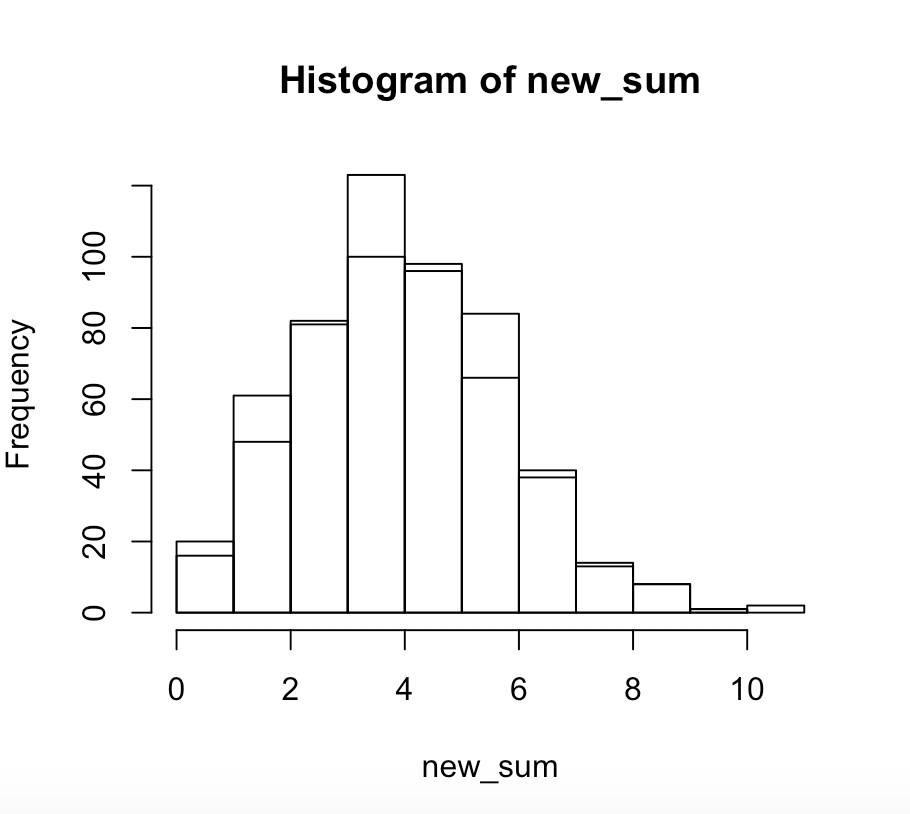
\includegraphics[scale=.65]{HISTO}


PROGRAMMING PROBLEM 2
\begin{lstlisting}
X=rexp(5000, rate = 1)
Y=rexp(5000, rate = 1)
W=Y/X

invcdf <- function(r) {1/(1-r)}-1
rands=runif(5000)
Wdev=invcdf(rands)

W = sort(W)
W = W[1:4750]

Wdev = sort(Wdev)
Wdev = Wdev[1:4750]

plot(W, Wdev)
\end{lstlisting} 
\includegraphics[scale=.65]{SCATTER}
\end{document}